% =====================================================================================
% Apresentação da Entrega 1 -- Proposta e Análise Exploratória dos Dados
% Beamer 16:9 | português do Brasil | citações e referências em APA 7 (biblatex-apa)
% Compilação:  pdflatex apresentacao && biber apresentacao && pdflatex apresentacao && pdflatex apresentacao
% =====================================================================================
\documentclass[aspectratio=169,11pt]{beamer}

\usepackage[utf8]{inputenc}
\usepackage[T1]{fontenc}
\usepackage{lmodern}
\usepackage[brazilian]{babel}
\usepackage{csquotes}
\usepackage[style=apa,backend=biber]{biblatex}
\DeclareLanguageMapping{brazilian}{brazilian-apa}
\addbibresource{../relatorio/referencias.bib}
\usepackage{booktabs,graphicx,amsmath,amssymb,xspace,tikz}
\usetikzlibrary{arrows.meta,positioning,decorations.pathreplacing}
\graphicspath{{../figuras/}}

% Gerado automaticamente por codigo/piloto_eda.py -- não editar à mão.
\newcommand{\PilotoRho}{0,90\xspace}
\newcommand{\PilotoMedia}{9,112\xspace}
\newcommand{\PilotoDp}{1,166\xspace}
\newcommand{\PilotoCv}{12,8\xspace}
\newcommand{\PilotoAssim}{1,34\xspace}
\newcommand{\PilotoShapW}{0,891\xspace}
\newcommand{\PilotoShapP}{0,005\xspace}
\newcommand{\PilotoTeo}{9,00\xspace}
\newcommand{\PilotoErro}{1,2\xspace}
\newcommand{\PilotoIcInf}{8,68\xspace}
\newcommand{\PilotoIcSup}{9,55\xspace}
\newcommand{\PilotoZeroEmp}{10,4\xspace}
\newcommand{\PilotoZeroTeo}{10\xspace}
\newcommand{\PilotoLagum}{0,99\xspace}
\newcommand{\PilotoLagdez}{0,90\xspace}
\newcommand{\PilotoPnoventa}{44,2\xspace}
\newcommand{\PilotoMaximo}{64,0\xspace}
\newcommand{\PilotoTempo}{0,45\xspace}
\newcommand{\PilotoLnAssim}{0,96\xspace}
\newcommand{\PilotoLnShapP}{0,058\xspace}
\newcommand{\RepLagum}{0,22\xspace}
\newcommand{\RepLagumP}{0,25\xspace}
\newcommand{\WelchIniMedia}{7,42\xspace}
\newcommand{\WelchPlatoMedia}{8,90\xspace}
\newcommand{\WelchDifPct}{$-$16,6\xspace}
\newcommand{\WelchResidDif}{$-$0,12\xspace}
\newcommand{\WelchResidEp}{0,36\xspace}
\newcommand{\CompCurtoCv}{17,2\xspace}
\newcommand{\CompCurtoMeia}{12,3\xspace}
\newcommand{\CompLongoCv}{12,8\xspace}
\newcommand{\CompLongoMeia}{9,2\xspace}
\newcommand{\TempoTotalEstimado}{36\xspace}
\newcommand{\NClientes}{50.000\xspace}
\newcommand{\NCurto}{10.000\xspace}
\newcommand{\Aquecimento}{1.000\xspace}
\newcommand{\RPiloto}{30\xspace}
\newcommand{\RWelch}{300\xspace}
\newcommand{\NWelch}{6.000\xspace}
\newcommand{\JanelaWelch}{250\xspace}

% Gerado por codigo/verificacao_simulador.py
\newcommand{\VerifMaxErro}{1,3\xspace}
\newcommand{\VerifNLongo}{400.000\xspace}
\newcommand{\VerifReps}{5\xspace}

% Recursos de hardware do ambiente onde o piloto foi executado.
% >>> Se as corridas finais forem executadas em outra máquina, edite estas linhas. <<<
\newcommand{\HwCPU}{Intel(R) Xeon(R) Processor @ 2.10GHz}
\newcommand{\HwNucleos}{1}
\newcommand{\HwRAM}{3,9}
\newcommand{\HwSO}{Linux 6.18.44-fc-v37}
\newcommand{\SwTeX}{pdfTeX 3.141592653-2.6-1.40.25 (TeX Live 2023/Debian)}
\newcommand{\SwBiber}{2.19}

\newcommand{\Wq}{W_q}

% ------------------------------------------------------------------------- aparência
\definecolor{azul}{RGB}{31,78,121}
\definecolor{laranja}{RGB}{197,90,17}
\setbeamercolor{structure}{fg=azul}
\setbeamercolor{frametitle}{fg=azul}
\setbeamercolor{footline}{fg=gray}
\setbeamertemplate{navigation symbols}{}
\setbeamertemplate{itemize items}[circle]
\setbeamertemplate{enumerate items}[default]
\setbeamerfont{itemize/enumerate body}{size=\normalsize}
\setbeamerfont{itemize/enumerate subbody}{size=\small}
\setbeamertemplate{frametitle}{%
  \vskip1.0ex
  \begin{beamercolorbox}[wd=\paperwidth,leftskip=1.2em]{frametitle}
    \usebeamerfont{frametitle}\insertframetitle\strut
    \vskip0.4ex
    \hrule height 0.8pt
  \end{beamercolorbox}}
\setbeamerfont{frametitle}{series=\bfseries,size=\large}
\setbeamertemplate{footline}{%
  \leavevmode\hbox{\begin{beamercolorbox}[wd=\paperwidth,ht=2.5ex,dp=1ex,leftskip=1.2em,rightskip=1.2em]{footline}%
    \usebeamerfont{footline}\scriptsize Sanchez Morales, G. A. - Benites Rodriguez, C. F.\hfill Experimento fatorial em filas simuladas\hfill \insertframenumber{} / \inserttotalframenumber
  \end{beamercolorbox}}}
\setbeamertemplate{bibliography item}{}
\setlength{\leftmargini}{1.2em}

% Rótulos ao estilo APA (número em negrito, título em itálico, nota abaixo)
\newcounter{figslide}\newcounter{tabslide}
\newcommand{\figcap}[1]{{\footnotesize\stepcounter{figslide}\textbf{Figura \thefigslide}\\\textit{#1}}\par\vspace{2pt}}
\newcommand{\tabcap}[1]{{\footnotesize\stepcounter{tabslide}\textbf{Tabela \thetabslide}\\\textit{#1}}\par\vspace{2pt}}
\newcommand{\nota}[1]{\par\vspace{3pt}{\scriptsize\textit{Nota.} #1}\par}
\newcommand{\destaque}[1]{{\color{azul}\bfseries #1}}

\title{Desempenho de Sistemas de Filas Simulados}
\author{Gruner Antonio Sanchez Morales - Carlos Fabricio Benites Rodriguez}
\date{21 de setembro de 2026}

\begin{document}

% ------------------------------------------------------------------------- 1. título
\begin{frame}[plain]
  \vspace*{1.3cm}
  {\color{azul}\LARGE\bfseries Desempenho de Sistemas de Filas Simulados:\par}
  \vspace{2pt}
  {\color{azul}\Large Proposta de Experimento Fatorial $2^3$ com Replicações\\e Análise Exploratória dos Dados\par}
  \vspace{0.9cm}
  {\large Gruner Antonio Sanchez Morales - Carlos Fabricio Benites Rodriguez\par}
  \vspace{4pt}
  Departamento de Computação, Universidade Federal de Ouro Preto\par
  Projeto e Análise de Experimentos Computacionais --- Entrega 1\par
  21 de setembro de 2026
\end{frame}

% ------------------------------------------------------------------------- 2. roteiro
\begin{frame}{Roteiro}
  \begin{enumerate}
    \setlength{\itemsep}{5pt}
    \item Contextualização e problema
    \item Objetivo e hipótese geral
    \item Estrutura experimental e projeto fatorial $2^3 r$
    \item Fonte dos dados e ambiente computacional
    \item Análise exploratória dos dados (piloto)
    \item Viabilidade, decisões de projeto e próximos passos
  \end{enumerate}
\end{frame}

% ------------------------------------------------------------------------- 3. contexto
\begin{frame}{Contextualização: por que estudar filas?}
  \begin{itemize}
    \setlength{\itemsep}{6pt}
    \item Filas surgem quando uma demanda variável disputa recursos limitados: requisições em servidores, pacotes em roteadores, processos em uma CPU, clientes em um guichê.
    \item Decisão típica de projeto: \destaque{quantos servidores} alocar para uma carga esperada \parencite{jain1991}.
    \item A teoria de filas dá fórmulas fechadas só em casos particulares; a \destaque{simulação de eventos discretos} cobre o restante \parencite{law2000}.
    \item Cada corrida de simulação é aleatória: trata-se de um \destaque{experimento computacional}, que exige planejamento (fatores, replicações, aleatorização) \parencite{jain1991,montgomery2017}.
  \end{itemize}
\end{frame}

% ------------------------------------------------------------------------- 4. sistema e problema
\begin{frame}{Sistema estudado e problema}
  \figcap{Sistema de filas modelado}
  \centering
  \begin{tikzpicture}[>=Stealth, font=\small, every node/.style={inner sep=3pt}, scale=0.92, transform shape]
    \node[draw,rounded corners,align=center,minimum height=1.1cm,minimum width=2.3cm] (src) at (0,0) {Chegadas\\Poisson($\lambda$)};
    \foreach \i in {0,1,2,3} \node[draw,minimum width=0.55cm,minimum height=1.0cm] (q\i) at (3.3+0.55*\i,0) {};
    \node[above=3pt of q1.north east,font=\footnotesize] {Fila FIFO};
    \node[draw,circle,minimum size=0.95cm] (s1) at (7.4,0.85) {$1$};
    \node[draw,circle,minimum size=0.95cm] (sc) at (7.4,-0.85) {$c$};
    \node at (7.4,0) {$\vdots$};
    \node[font=\footnotesize,align=center] at (7.4,1.85) {tempo de serviço $S$\\(média de 1 min)};
    \node[draw,rounded corners,minimum height=1.1cm,minimum width=1.6cm] (out) at (10.6,0) {Saídas};
    \draw[->] (src) -- (q0.west);
    \draw[->] (q3.east) -- (s1.west);
    \draw[->] (q3.east) -- (sc.west);
    \draw[->] (s1.east) -- ++(0.9,0) |- (out.north west);
    \draw[->] (sc.east) -- ++(0.9,0) |- (out.south west);
    \draw[decorate,decoration={brace,amplitude=4pt,mirror}] (3.0,-0.65) -- node[below=4pt,font=\footnotesize]{espera $\Wq$} (5.25,-0.65);
  \end{tikzpicture}
  \vspace{8pt}

  \begin{flushleft}
  \destaque{Problema:} como o número de servidores, a intensidade de chegadas e a variabilidade do serviço afetam --- isolada e conjuntamente --- a espera média em fila em regime estacionário?

  \vspace{4pt}
  \destaque{Relevância:} orienta o dimensionamento de capacidade; a espera responde de forma não linear à utilização, o que sugere \destaque{interações}.
  \end{flushleft}
\end{frame}

% ------------------------------------------------------------------------- 5. objetivo
\begin{frame}{Objetivo}
  \destaque{Objetivo geral.} Avaliar, com um projeto fatorial $2^3$ e $r = 10$ replicações, o efeito do número de servidores, da taxa de chegada e da distribuição do tempo de serviço sobre a espera média em fila.

  \vspace{8pt}
  \destaque{Objetivos específicos}
  \begin{enumerate}
    \setlength{\itemsep}{4pt}
    \item Estimar efeitos principais e interações, com intervalos de confiança.
    \item Determinar a proporção da variação atribuída a cada fator, interação e ao erro.
    \item Verificar as suposições do modelo (normalidade, variância constante, independência) e decidir sobre uma transformação.
    \item Garantir reprodutibilidade completa: código, sementes e versões registrados.
  \end{enumerate}
\end{frame}

% ------------------------------------------------------------------------- 6. hipótese
\begin{frame}{Hipótese geral do estudo}
  \destaque{Definida antes da execução} do experimento fatorial:
  \begin{itemize}
    \setlength{\itemsep}{4pt}
    \item Mais servidores (A) $\Rightarrow$ \destaque{menor} espera.
    \item Maior taxa de chegada (B) $\Rightarrow$ \destaque{maior} espera.
    \item Serviço constante, sem variabilidade (C) $\Rightarrow$ \destaque{menor} espera.
    \item Efeitos de A e de C \destaque{mais intensos sob alta carga}: interações A$\times$B e B$\times$C.
  \end{itemize}
  \vspace{6pt}
  Base teórica (fila M/G/1) \parencite{jain1991}:
  \[
    \Wq = \frac{\rho\,(1 + c_s^2)}{2\mu\,(1-\rho)}
  \]
  \vspace{-4pt}
  Expectativa \destaque{teórica}, formulada antes das corridas: não vem do piloto e só será avaliada com o fatorial completo (Entrega 2).
\end{frame}

% ------------------------------------------------------------------------- 7. estrutura
\begin{frame}{Estrutura experimental}
  \begin{columns}[T]
    \begin{column}{0.52\textwidth}
      \destaque{Unidade experimental}\\
      Uma corrida independente: \NClientes{} clientes, semente própria, sistema inicialmente vazio.

      \vspace{8pt}
      \destaque{Variável de resposta}\\
      Espera média em fila por corrida (min), após o aquecimento:
      \[
        \overline{W}_q = \frac{1}{N - W}\sum_{i=W+1}^{N} W_{q,i}
      \]
      com $N = $ \NClientes{} e $W = $ \Aquecimento{}.
    \end{column}
    \begin{column}{0.44\textwidth}
      \destaque{Condições constantes}
      \begin{itemize}
        \setlength{\itemsep}{2pt}
        \item Tempo médio de serviço: 1 min
        \item Disciplina FIFO; fila infinita; sem abandono
        \item Chegadas de Poisson
        \item Mesmos $N$, $W$, código e versões
        \item Mesma máquina, sem outras cargas pesadas
      \end{itemize}
    \end{column}
  \end{columns}
\end{frame}

% ------------------------------------------------------------------------- 8. fatores
\begin{frame}{Fatores e níveis}
  \centering
  \tabcap{Fatores e níveis do experimento}
  \begin{tabular}{llcc}
    \toprule
    Fator & Descrição & Nível $-1$ & Nível $+1$ \\
    \midrule
    A & Número de servidores ($c$) & 1 & 2 \\
    B & Taxa de chegada ($\lambda$, clientes/min) & 0,5 & 0,9 \\
    C & Distribuição do tempo de serviço & Exponencial & Constante \\
    \bottomrule
  \end{tabular}
  \nota{Em ambos os níveis de C a média do serviço é 1 min; a exponencial tem $c_s = 1$ e a constante tem $c_s = 0$.}

  \vspace{10pt}
  \begin{flushleft}
  Em todas as combinações a utilização é $\rho < 1$ (de 0,25 a 0,90): existe regime estacionário.
  \end{flushleft}
\end{frame}

% ------------------------------------------------------------------------- 9. aleatorização
\begin{frame}{Procedimento de aleatorização}
  \begin{enumerate}
    \setlength{\itemsep}{8pt}
    \item \destaque{Sementes independentes:} cada uma das 80 corridas recebe um fluxo próprio com \texttt{SeedSequence.spawn} (NumPy), gerador PCG64 \parencite{oneill2014}.
    \item \destaque{Ordem aleatória:} a ordem de execução das 80 corridas é uma permutação uniforme, com semente própria, para não confundir efeitos de ordem com os fatores.
    \item \destaque{Plano prévio:} o plano completo é gerado e guardado \emph{antes} de qualquer corrida do experimento.
  \end{enumerate}
\end{frame}

% ------------------------------------------------------------------------- 10. fatorial
\begin{frame}{Projeto fatorial $2^3 r$: as 8 combinações}
  \begin{columns}[T]
    \begin{column}{0.58\textwidth}
      \tabcap{Combinações experimentais ($r = 10$ por combinação)}
      \resizebox{\textwidth}{!}{\begin{tabular}{cccccccc}
\toprule
Célula & $A$ & $B$ & $C$ & $c$ & $\lambda$ (cl/min) & Serviço & $\rho$ \\
\midrule
1 & $-$ & $-$ & $-$ & 1 & 0,5 & exponencial & 0,50 \\
2 & $+$ & $-$ & $-$ & 2 & 0,5 & exponencial & 0,25 \\
3 & $-$ & $+$ & $-$ & 1 & 0,9 & exponencial & 0,90 \\
4 & $+$ & $+$ & $-$ & 2 & 0,9 & exponencial & 0,45 \\
5 & $-$ & $-$ & $+$ & 1 & 0,5 & constante & 0,50 \\
6 & $+$ & $-$ & $+$ & 2 & 0,5 & constante & 0,25 \\
7 & $-$ & $+$ & $+$ & 1 & 0,9 & constante & 0,90 \\
8 & $+$ & $+$ & $+$ & 2 & 0,9 & constante & 0,45 \\
\bottomrule
\end{tabular}
}
      \nota{$\rho = \lambda/(c\mu)$. Total: $8 \times 10 = 80$ corridas.}
    \end{column}
    \begin{column}{0.4\textwidth}
      \small
      \destaque{Modelo} \parencite{jain1991}
      \[
        y = q_0 + \sum_j q_j x_j + \sum_{j<k} q_{jk}x_j x_k + q_{ABC}x_Ax_Bx_C + e
      \]
      \destaque{Análise (após as corridas)}
      \begin{itemize}
        \setlength{\itemsep}{1pt}
        \item Efeitos e alocação da variação
        \item ANOVA e IC de 95\%
        \item Diagnóstico de resíduos
        \item Transformação, se necessário \parencite{box1964}
      \end{itemize}
    \end{column}
  \end{columns}
\end{frame}

% ------------------------------------------------------------------------- 11. dados
\begin{frame}{Fonte dos dados: simulação verificada}
  \begin{itemize}
    \setlength{\itemsep}{5pt}
    \item Dados \destaque{gerados por simulação} de eventos discretos em SimPy \parencite{simpy}: cada cliente é um processo que solicita um servidor (\texttt{Resource}, fila FIFO).
    \item Entre chegadas exponenciais; serviço exponencial ou constante; números aleatórios gerados antes da corrida (a semente determina a corrida).
    \item \destaque{Verificação contra a teoria:} Pollaczek--Khinchine (M/M/1, M/D/1) e Erlang C (M/M/2), com \VerifReps{} corridas de \VerifNLongo{} clientes em seis combinações. \destaque{Erro relativo máximo: \VerifMaxErro{}\%.}
    \item Limitação: M/D/2 não tem fórmula fechada simples; usa o mesmo código das combinações verificadas.
  \end{itemize}
\end{frame}

% ------------------------------------------------------------------------- 12. ambiente
\begin{frame}{Ambiente computacional e reprodutibilidade}
  \begin{columns}[T]
    \begin{column}{0.36\textwidth}
      \tabcap{Versões de software}
      \footnotesize
      \begin{tabular}{ll}
\toprule
Componente & Versão \\
\midrule
Python & 3.14.4 \\
SimPy & 4.1.2 \\
NumPy & 2.4.4 \\
SciPy & 1.17.1 \\
pandas & 3.0.2 \\
statsmodels & 0.15.0 \\
Matplotlib & 3.10.8 \\
\bottomrule
\end{tabular}

      \nota{Fixadas em \texttt{requirements.txt}.}
    \end{column}
    \begin{column}{0.60\textwidth}
      \small
      Bibliotecas: SimPy \parencite{simpy}, NumPy \parencite{harris2020}, SciPy \parencite{virtanen2020}, statsmodels \parencite{seabold2010}, pandas \parencite{mckinney2010}, Matplotlib \parencite{hunter2007}.

      \vspace{4pt}
      Hardware do piloto: \HwCPU{}, \HwNucleos{} núcleo(s), \HwRAM{} GB, \HwSO{}.

      \vspace{4pt}
      \destaque{Ambiente controlado} \parencite{sandve2013,wilson2017}:
      \begin{itemize}
        \setlength{\itemsep}{1pt}
        \item Versões e sementes registradas
        \item Execução só por \emph{scripts}, sem passos manuais
        \item Dados brutos das 80 corridas preservados
        \item Uma máquina, sem outras cargas
        \item 80 corridas $\approx$ \TempoTotalEstimado{} s; sem APIs nem LLMs
      \end{itemize}
    \end{column}
  \end{columns}
\end{frame}

% ------------------------------------------------------------------------- 12b. cuidados metodológicos
\begin{frame}{Cuidados metodológicos para evitar erros}
  \small
  \begin{tabular}{@{}p{0.36\textwidth}p{0.58\textwidth}@{}}
    \toprule
    \textbf{Risco} & \textbf{Como o estudo o evita} \\
    \midrule
    Confundir a hipótese com achados da AED & Hipótese formulada \emph{antes}, a partir da teoria de filas; a AED não a avalia. \\[4pt]
    Antecipar conclusões do fatorial na AED & Piloto em \destaque{uma única configuração}; não compara níveis nem estima efeitos. \\[4pt]
    Réplicas que não são independentes & Cada réplica é uma \destaque{execução completa} (sistema vazio, semente nova); não são lotes de uma corrida nem clientes consecutivos. Independência verificada no piloto. \\[4pt]
    Execuções incompatíveis com o hardware & $8 \times 10 = 80$ corridas, cerca de \TempoTotalEstimado{} s no total; sem APIs nem modelos de linguagem, logo sem cotas. \\
    \bottomrule
  \end{tabular}
\end{frame}

% ------------------------------------------------------------------------- 13. EDA: desenho do piloto
\begin{frame}{Análise exploratória: desenho do piloto}
  \begin{itemize}
    \setlength{\itemsep}{6pt}
    \item Corridas piloto com \destaque{sementes diferentes} das do experimento; não entram na análise fatorial.
    \item \destaque{Uma única configuração}, escolhida a priori: célula 3 ($c = 1$, $\lambda = 0{,}9$, serviço exponencial; $\rho = \PilotoRho{}$), a mais exigente para dimensionar as corridas \parencite{kelton1985,law2000}.
    \item \RPiloto{} corridas independentes, cada uma completa, com $N = $ \NClientes{} e $W = $ \Aquecimento{}.
    \item Propósito: \destaque{caracterizar a resposta e avaliar a viabilidade}.
    \item Não compara níveis dos fatores, não estima efeitos e \destaque{não avalia a hipótese}.
  \end{itemize}
\end{frame}

% ------------------------------------------------------------------------- 14. EDA: estatísticas descritivas
\begin{frame}{Estatísticas descritivas: médias por corrida}
  \begin{columns}[T]
    \begin{column}{0.48\textwidth}
      \tabcap{Médias por corrida no piloto ($n = \RPiloto{}$)}
      \small
      \begin{tabular}{lr}
        \toprule
        Estatística & Valor \\
        \midrule
        Média (min) & \PilotoMedia{} \\
        Desvio-padrão (min) & \PilotoDp{} \\
        Coef. de variação (\%) & \PilotoCv{} \\
        Assimetria & \PilotoAssim{} \\
        Shapiro--Wilk $W$ ($p$) & \PilotoShapW{} (\PilotoShapP{}) \\
        IC 95\% da média (min) & [\PilotoIcInf{}; \PilotoIcSup{}] \\
        \midrule
        Valor teórico (min) & \PilotoTeo{} \\
        Erro relativo (\%) & \PilotoErro{} \\
        \bottomrule
      \end{tabular}
      \nota{IC: intervalo de confiança de 95\%. Valor teórico: fórmula M/M/1. Quartis, mínimo e máximo estão no relatório.}
    \end{column}
    \begin{column}{0.48\textwidth}
      \small
      \begin{itemize}
        \setlength{\itemsep}{6pt}
        \item Média próxima da teoria; o IC contém o valor teórico.
        \item Dispersão entre corridas grande: CV de \PilotoCv{}\%.
        \item Distribuição \destaque{assimétrica à direita}: algumas corridas com espera média alta.
      \end{itemize}
    \end{column}
  \end{columns}
\end{frame}

% ------------------------------------------------------------------------- 15. EDA: esperas individuais
\begin{frame}{Distribuição das esperas individuais}
  \begin{columns}[c]
    \begin{column}{0.56\textwidth}
      \figcap{Esperas individuais (primeira corrida piloto)}
      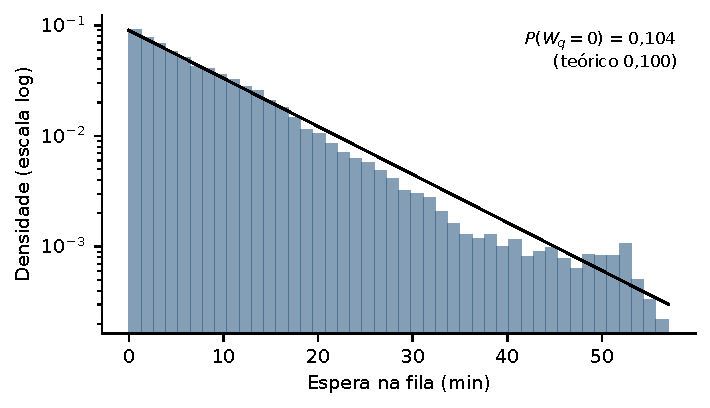
\includegraphics[width=\textwidth]{fig_esperas_individuais}
      \nota{Esperas positivas, escala log; linha preta: densidade teórica M/M/1.}
    \end{column}
    \begin{column}{0.40\textwidth}
      \small
      \begin{itemize}
        \setlength{\itemsep}{6pt}
        \item Massa de probabilidade em zero e cauda exponencial.
        \item $P(\Wq = 0)$ empírica de \PilotoZeroEmp{}\% (teórica: \PilotoZeroTeo{}\%).
        \item Em 1\% dos casos a espera passa de \PilotoPnoventa{} min.
      \end{itemize}
    \end{column}
  \end{columns}
\end{frame}

% ------------------------------------------------------------------------- 16. EDA: médias por corrida
\begin{frame}{Distribuição das médias por corrida}
  \begin{columns}[c]
    \begin{column}{0.63\textwidth}
      \figcap{Médias por corrida no piloto}
      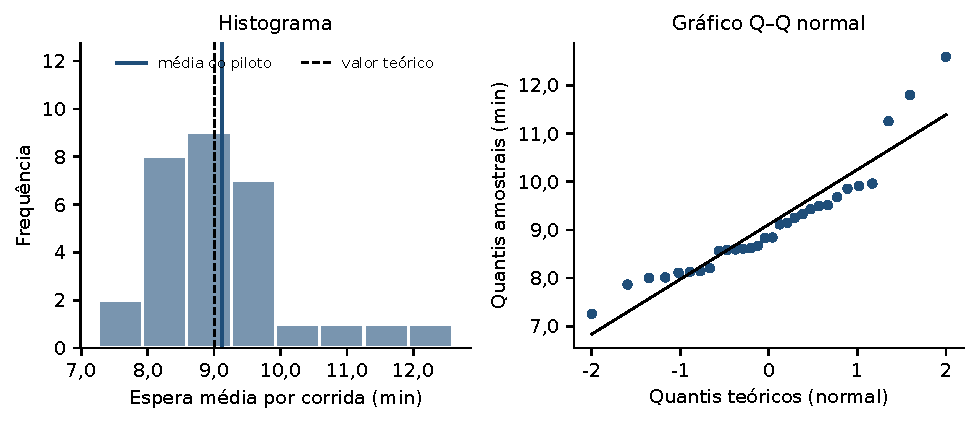
\includegraphics[width=\textwidth]{fig_distribuicao_medias}
    \end{column}
    \begin{column}{0.33\textwidth}
      \small
      \begin{itemize}
        \setlength{\itemsep}{5pt}
        \item Shapiro--Wilk \parencite{shapiro1965} \destaque{rejeita} a normalidade: $p = \PilotoShapP{}$.
        \item Q--Q: afastamento na cauda superior.
        \item Em escala log: assimetria \PilotoLnAssim{}, $p = \PilotoLnShapP{}$ (poder limitado).
        \item Não decide a análise: indica \destaque{verificar os resíduos} no experimento.
      \end{itemize}
    \end{column}
  \end{columns}
\end{frame}

% ------------------------------------------------------------------------- 17. EDA: independência (réplicas) e dependência (clientes)
\begin{frame}{Réplicas independentes; clientes dependentes}
  \begin{columns}[T]
    \begin{column}{0.49\textwidth}
      \figcap{Média por corrida segundo a ordem das réplicas}
      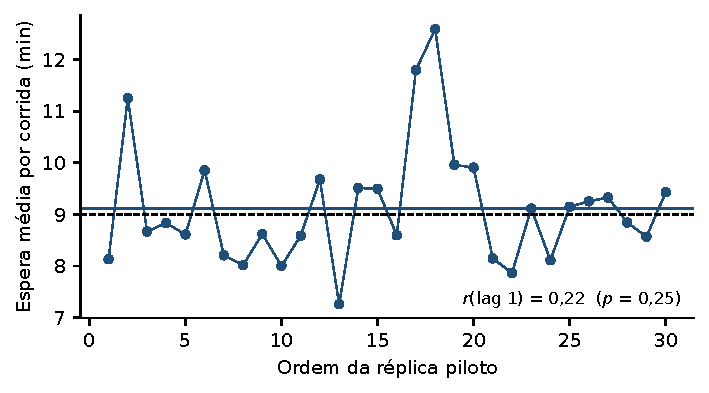
\includegraphics[width=\textwidth]{fig_replicas}
    \end{column}
    \begin{column}{0.49\textwidth}
      \figcap{Autocorrelação das esperas individuais}
      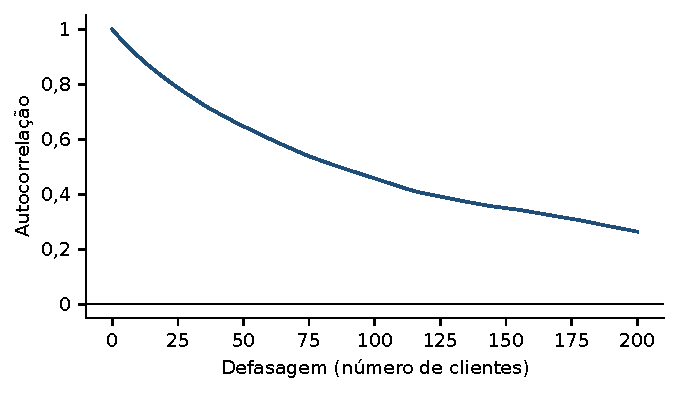
\includegraphics[width=\textwidth]{fig_acf}
    \end{column}
  \end{columns}
  \vspace{4pt}
  \small
  \begin{itemize}
    \setlength{\itemsep}{2pt}
    \item \destaque{Réplicas:} sem tendência; correlação entre réplicas consecutivas $r = \RepLagum{}$ ($p = \RepLagumP{}$). Esperado: cada réplica é uma execução completa com semente própria.
    \item \destaque{Clientes:} autocorrelação de \PilotoLagum{} (defasagem 1) e \PilotoLagdez{} (defasagem 10): esperas individuais não são independentes; a unidade de análise é a média por corrida.
  \end{itemize}
\end{frame}

% ------------------------------------------------------------------------- 19. EDA: aquecimento
\begin{frame}{Período de aquecimento}
  \begin{columns}[c]
    \begin{column}{0.56\textwidth}
      \figcap{Procedimento gráfico de Welch}
      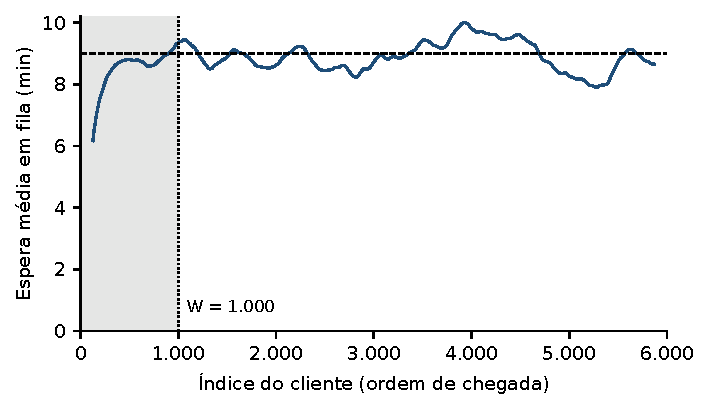
\includegraphics[width=\textwidth]{fig_welch}
      \nota{Média entre \RWelch{} réplicas, média móvel de \JanelaWelch{} clientes \parencite{welch1983}. Tracejado: valor teórico; cinza: aquecimento descartado.}
    \end{column}
    \begin{column}{0.40\textwidth}
      \small
      \begin{itemize}
        \setlength{\itemsep}{5pt}
        \item Os 500 primeiros clientes esperam \WelchDifPct{}\% em relação ao platô.
        \item A curva se estabiliza antes de 1.000 clientes.
        \item Com $W = $ \Aquecimento{}, a diferença residual é \WelchResidDif{} $\pm$ \WelchResidEp{} min: indistinguível de zero.
      \end{itemize}
    \end{column}
  \end{columns}
\end{frame}

% ------------------------------------------------------------------------- 20. viabilidade
\begin{frame}{Viabilidade e decisões de projeto}
  \centering
  \tabcap{Comprimento da corrida e dispersão da resposta (piloto, \RPiloto{} corridas por linha)}
  \resizebox{0.86\textwidth}{!}{\begin{tabular}{rrrrr}
\toprule
$N$ (clientes) & $s$ (min) & CV (\%) & Meia-largura do IC ($r=10$) & Tempo/corrida (s) \\
\midrule
10.000 & 1,508 & 17,2 & $\pm$ 12,3\% & 0,088 \\
50.000 & 1,166 & 12,8 & $\pm$ 9,2\% & 0,445 \\
\bottomrule
\end{tabular}
}
  \nota{Meia-largura do IC de 95\% para uma combinação com $r = 10$, em \% da média.}

  \vspace{4pt}
  \begin{flushleft}
  \small
  \destaque{Decisões:}
  (1) $N = $ \NClientes{} por corrida; (2) $W = $ \Aquecimento{} descartados; (3) média por corrida como unidade, com réplicas completas e independentes; (4) verificar normalidade e variâncias dos resíduos no experimento; (5) 80 corridas em cerca de \TempoTotalEstimado{} s, compatível com o hardware.
  \end{flushleft}
\end{frame}

% ------------------------------------------------------------------------- 21. próximos passos
\begin{frame}{Próximos passos e limitações}
  \begin{columns}[T]
    \begin{column}{0.48\textwidth}
      \destaque{Próximos passos}
      \begin{enumerate}
        \setlength{\itemsep}{4pt}
        \item Executar as 80 corridas na ordem sorteada
        \item Entrega 2 (26/10): efeitos, interações, IC e testes de significância
        \item Diagnóstico dos resíduos
        \item Avaliação preliminar da hipótese
      \end{enumerate}
    \end{column}
    \begin{column}{0.48\textwidth}
      \destaque{Limitações}
      \begin{itemize}
        \setlength{\itemsep}{4pt}
        \item Vale para chegadas de Poisson, fila infinita e serviço de média fixa
        \item $r = 10$ é o mínimo; pode aumentar (corridas baratas)
        \item M/D/2 sem verificação teórica exata
      \end{itemize}
    \end{column}
  \end{columns}
\end{frame}

% ------------------------------------------------------------------------- referências
\begin{frame}[allowframebreaks]{Referências}
  \footnotesize
  \printbibliography[heading=none]
\end{frame}

\end{document}
